%%% %%%%%%%%%%%%%%%%%%%%%%%%%%%%%%%%%%%%%%%%%%%%%%%%%%%%%%%%%%%%%%%%%%%%%%%%%%%% 

\rawhtml
<a name="production_code_program_synthesis"></a>
\endrawhtml
\subsectional{Generation: Automated Code Synthesis}

%%% %%%%%%%%%%%%%%%%%%%%%%%%%%%%%%%%%%%%%%%%%%%%%%%%%%%%%%%%%%%%%%%%%%%%%%%%%%%%

Gulwani~\etal{}~\cite{GulwanietalFaTiPL-17} provide an up-to-date survey of challenges and technologies in automated program synthesis. Machine learning is allocated only 10 of the more than 100 pages in the review with neural network-methods singled out as a separate section of 6 additional pages. My experience is that many current devotees are largely ignorant concerning the relevant history including the many successful applications for handling interesting special cases. I won't attempt to remedy that state of affairs here except to recommend that readers interested in program synthesis spend the time to familiarize themselves with the relevant work including both successes and notable failures. 

For those of you primarily interested in neural-network methods, understanding this background is likely to prove useful in developing hybrid systems that combine connectionist models and more conventional symbolic methods. Already, the power of high-dimensional vector-space representations, context-sensitive embedding spaces and fully-differentiable models trained with backpropagation is winning converts among advocates of more traditional methods, even as the latest generation of neural-network experts working on what is popularly called neural program synthesis are rediscovering some of the same special cases that have been exploited in deductive and constraint-based approaches to automated code synthesis.

%%% %%%%%%%%%%%%%%%%%%%%%%%%%%%%%%%%%%%%%%%%%%%%%%%%%%%%%%%%%%%%%%%%%%%%%%%%%%%%

\subsubsectional{Teaching}

%%% %%%%%%%%%%%%%%%%%%%%%%%%%%%%%%%%%%%%%%%%%%%%%%%%%%%%%%%%%%%%%%%%%%%%%%%%%%%%

Given the title, you might have expected that this document would be all about automatic programming, but it's really about human augmentation and human-computer collaboration. Programming is all about representing procedural knowledge in an interpretable form, i.e., executable on some computational substrate. Teaching someone to program or, for that matter, teaching someone to do most anything nontrivial, is also about representing and communicating procedural knowledge in an interpretable form \emdash{} the clearer and more precise the communication, the simpler and less knowledgeable the required substrate.

In this section, we attempt to identify special cases in which it is relatively easy for a human programmer to instruct an AI system how to facilitate the conversion of thoughts conveyed in natural language into working programs \emdash{} see Graham Neubig's CS379C calendar {\urlh{https://web.stanford.edu/class/cs379c/calendar_invited_talks/lectures/05/01/index.html}{page}} for a sample of his NLP work on code generation and learning dialog systems. We are not anticipating that we will be able to read minds so much as exploit shared knowledge in order to translate succinct descriptions of desired computations \emdash{} along with an implicit understanding of what constitutes a suitable computational solution \emdash{} into working software possibly with guarantees of its correctness and performance.

How does this perspective inform the discussion in this section? Prior to any training the apprentice comes equipped with a very basic language facility and an innate ability to work with computer programs, but the former is practically useless since the meta-learning controller hasn't been trained and the latter only produces results in the same way that a baby has virtually no control over its limbs and torso. It learns to communicate by reinforcement when it successfully carries out a command from the expert programmer. A built-in training system expedites this process and relieves some of the burden from the programmer by generating synthetic commands that serve to initialize the meta-learning controller allowing the assistant to achieve a basic facility for directly translating natural language commands exercising the integrated development environment.

The apprentice also comes pre-trained with a (semantic) {\urlh{https://en.wikipedia.org/wiki/Language_model}{language model}} trained on a corpus that includes a large vocabulary of practical and technical terms used by programmers in talking about programs and programming. The apprentice ingests a large corpus of programs and program fragments written in the language that it will use for writing new programs, resulting in an embedding space that encodes these programs and an encoder-decoder translation facility that allows it to read and write programs represented as abstract syntax trees. Were there more computer- / natural-language {\urlh{https://en.wikipedia.org/wiki/Parallel_text#Parallel_corpora}{parallel corpora}}, supervised training of systems that depend on natural-language specification as input would be tempting. As it is, we have to rely on more subtle strategies.

%%% %%%%%%%%%%%%%%%%%%%%%%%%%%%%%%%%%%%%%%%%%%%%%%%%%%%%%%%%%%%%%%%%%%%%%%%%%%%% 

Perhaps it is not surprising that many current neural-network approaches take advantage of neural-network technology originally designed for machine translation, question answering and related natural-language processing applications. Programs are linguistic objects with relatively simple syntax. Their syntax is well understood since linguistically adept computer scientists designed them. Parsing programs is trivial using standard compiler tools. Their semantics is revealed by running them, and not just their input-output behavior \emdash{} execution traces can be used to reveal the meaning of every function and fragment. 

Programming languages are syntactically unforgiving \emdash{} a source of aggravation for beginning programmers, but we have sophisticated editors and syntax checkers that avoid most problems and there is no reason not to build them into the integrated development environment used by the programmer's assistant and shared with the programmer. Internally, the assistant can work with equivalent abstract syntax trees making it easy to ingest, embed, manipulate and generate proposals for performing program transformations on such representations. Human readable code can be recovered for the programmer's convenience.

Successful code synthesis can be verified by running the program and comparing with the provided input-output examples. Modulo the intractability of the halting problem, failure for relatively simple programs can be easily determined. Program {\urlh{https://en.wikipedia.org/wiki/Correctness_(computer_science)}{correctness}} is generally specified with respect to a specification and hence is more difficult to pin down, though the term generally implies the existence of a mathematical proof and, hence, one formal-methods approach to code synthesis involves generating a {\urlh{https://en.wikipedia.org/wiki/Constructive_proof}{constructive proof}} of correctness. 

Semantic embeddings are increasingly common~\cite{DevlinetalICLR-18,ChistyakovetalICLR-17,WangetalCoRR-17,XuetalCoRR-17,PiechetalICML-15} based on {\urlh{https://en.wikipedia.org/wiki/Software_diagnosis#Characteristics}{execution traces}}, {\urlh{https://en.wikipedia.org/wiki/Log_file#Event_logs}{event logs}}, or {\urlh{https://en.wikipedia.org/wiki/Invariant_(computer_science)}{program invariants}}. See this discussion log {\urlh{https://web.stanford.edu/class/cs379c/class_messages_listing/index.html#program_embedding_core_technology}{entry}} and Rishabh Singh's CS379C calendar {\urlh{https://web.stanford.edu/class/cs379c/calendar_invited_talks/lectures/05/24/index.html}{page}} plus this discussion log {\urlh{https://web.stanford.edu/class/cs379c/class_messages_listing/index.html#execution_logs_program_traces}{entry}} and Dawn Song's CS379C calendar {\urlh{https://web.stanford.edu/class/cs379c/calendar_invited_talks/lectures/05/31/index.html}{page}} for more on semantic embeddings. I'm not going into detail here for the simple reason that it is still early days and your best approach to learn more is to read the papers, check out the slides and watch the videos mentioned in this paragraph and at the end of this section \emdash{} you might also take a look at Danny Tarlow's list of selected program synthesis papers {\urlh{./content/Selected_Program_Synthesis_Papers_Tarlow.pdf}{here}}.

%%% %%%%%%%%%%%%%%%%%%%%%%%%%%%%%%%%%%%%%%%%%%%%%%%%%%%%%%%%%%%%%%%%%%%%%%%%%%%% 

\subsubsectional{Projects}

%%% %%%%%%%%%%%%%%%%%%%%%%%%%%%%%%%%%%%%%%%%%%%%%%%%%%%%%%%%%%%%%%%%%%%%%%%%%%%% 

In the Spring 2018 instance of Stanford {\urlh{https://web.stanford.edu/class/cs379c/}{CS379C}}, 30 students, organized in 12 teams proposed and carried out projects relating to the programmer's apprentice. As an example, the team consisting of Marcus Gomez, Nate Gruver, Michelle Lam, Rohun Saxena and Lucy Wang~\cite{CS379C_Final_Project_Gomezetal-18} decided based on their coding habits that the most helpful assistant would be one that could be trained to understand design through the structure of an application programming interface ({\urlh{https://en.wikipedia.org/wiki/Application_programming_interface}{API}}) and assist in the completion of the code through a divide-and-conquer approach {\urlh{./content/CS379C_Final_Project_Gomezetal-18.pdf}{PDF}}.

%%% %%%%%%%%%%%%%%%%%%%%%%%%%%%%%%%%%%%%%%%%%%%%%%%%%%%%%%%%%%%%%%%%%%%%%%%%%%%% 

\setcounter{figure}{2}

%%% %%%%%%%%%%%%%%%%%%%%%%%%%%%%%%%%%%%%%%%%%%%%%%%%%%%%%%%%%%%%%%%%%%%%%%%%%%%% 

%%% Figure~{\urlh{#fig_CS379C_Final_Project_Gomezetal_Figure_03}{3}}
\rawhtml
<a name="fig_CS379C_Final_Project_Gomezetal_Figure_03"></a>
\endrawhtml
\begin{figure}
%
  \hrule{}
%
  \begin{center}
    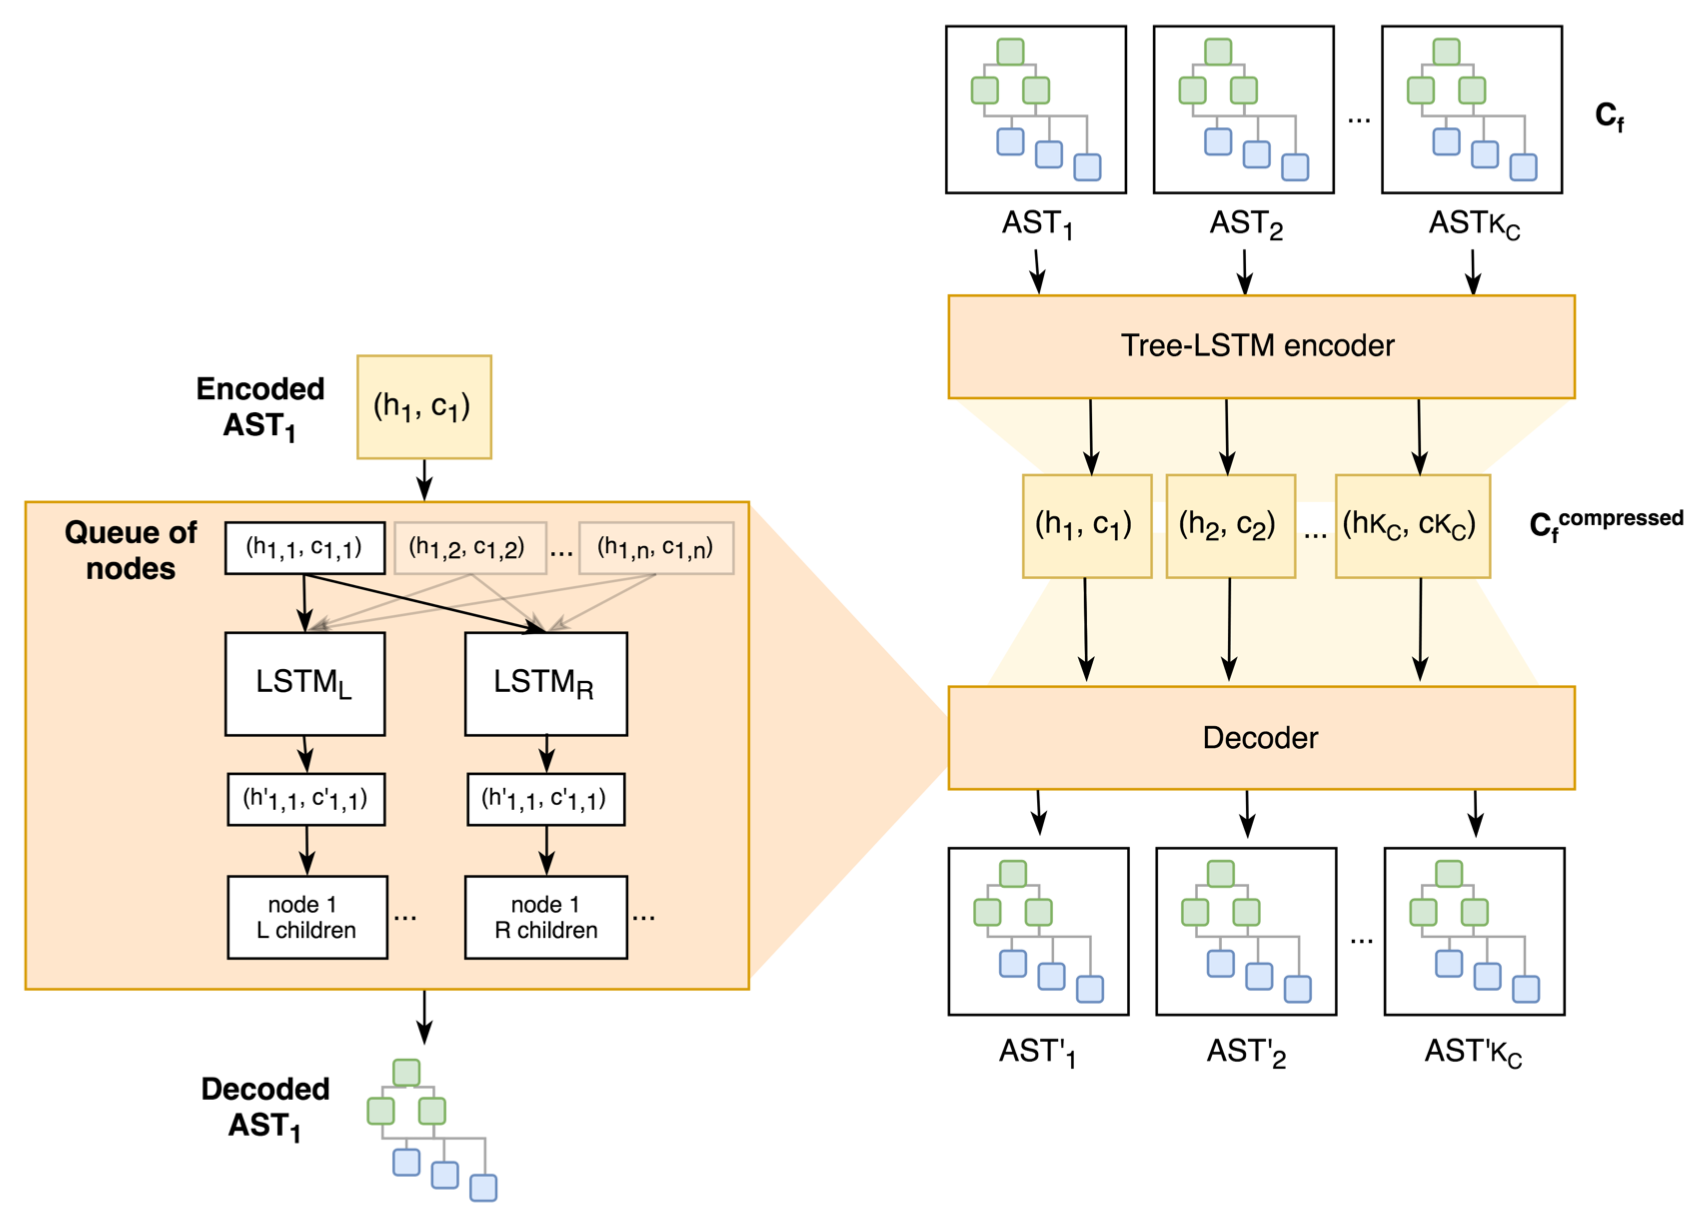
\includegraphics[width=10.0in]{./figures/CS379C_Final_Project_Gomezetal_Figure_03.png}
  \end{center}
%
  \caption{Summary of the proposed LSTM-based state-embedding architecture for $C_{f}$ described in Gomez~\etal{}~\cite{CS379C_Final_Project_Gomezetal-18}. The code representation, $C_{f}$, is by default variable in size since the abstract syntax trees that comprise the individual helper functions are variable size. The authors solve this problem by training an autoencoder penalized on reconstruction loss such that the decoded output is the binary tree representation of the original AST.}
%
  \hrule{}
%
\end{figure}

%%% %%%%%%%%%%%%%%%%%%%%%%%%%%%%%%%%%%%%%%%%%%%%%%%%%%%%%%%%%%%%%%%%%%%%%%%%%%%%

The system they envision would be designed to integrate seamlessly into programmer's workflow, minimize interaction and start from a simple header file and dependency graph. They took pains to standardize the format of the input in order to simplify learning a compressed fixed-size state vector as an ordered list of GLoVe vectors~\cite{PenningtonetalEMNLP-14} \emdash{} see Figure~{\urlh{#fig_CS379C_Final_Project_Gomezetal_Figure_03}{3}}. They employ the method of {\it{generative adversarial imitation learning}} (GAIL) developed by Ho and Ermon~\cite{HoandErmonCoRR-16} to extract a policy from data as if it were obtained by reinforcement learning following inverse reinforcement learning. GAIL should enable them to derive a model-free imitation-learning algorithm that obtains significant performance gains over existing model-free methods in imitating complex behaviors in large, high-dimensional environments.

%%% %%%%%%%%%%%%%%%%%%%%%%%%%%%%%%%%%%%%%%%%%%%%%%%%%%%%%%%%%%%%%%%%%%%%%%%%%%%%

Episodic memory is an important component of the programmer's apprentice. In order to exploit what you've learned through experience and previously consolidated in episodic memory, it is often necessary to reconstruct memories in enough detail that you can compare the past with current experience, determine if activities applied to resolve problems in the past apply in the present, and, if necessary, adapt those early responses to fit the present circumstances. Catherine Wong, in her final project report~\cite{CS379C_Final_Project_Wong-18} for CS379C, developed a new neural-network model for content-based and selectively-reconstructive memory inspired by research on {\it{hippocampal indexing theory}}~\cite{TeylerandRudyHIPPOCAMPUS-07} and {\it{adaptive deconvolutional networks}}~\cite{ZeileretalICCV-11,ZeileretalCVPR-10} {\urlh{./content/CS379C_Final_Project_Wong-18.pdf}{PDF}}. 

In designing her model she built upon the Kavukcuoglu~\etal{}~\cite{KavukcuogluetalNIPS-10} work on {\urlh{http://koray.kavukcuoglu.org/research.html}{convolutional predictive sparse decomposition}} and Kingma and Welling~\cite{KingmaandWellingCoRR-13} on {\urlh{https://www.ibm.com/blogs/research/2018/05/disentanglement-deep-learning/}{explicit feature disentanglement using variational autoencoders}}. While previous work has focused on deciding {\it{how}} to remember~\cite{WayneetalCoRR-18}, Catherine's model emphasizes deciding {\it{what}} to remember, focusing on the problem of leveraging compressive coding to balance the demands of efficient and effective content-based lookup with domain specificity. Her work is also closely related to and consistent with recent research~\cite{LatchoumaneetalNEURON-17,FanetalJCN-17,NielsenNLM-15} on the role of high-frequency {\urlh{https://en.wikipedia.org/wiki/Sleep_spindle}{thalamic sleep spindles}} during sleep-dependent memory consolidation\footnote{%
%
  For an introduction to the role of sleep in memory, check out the {\urlh{https://www.youtube.com/watch?v=stXhGMVJuqA}{video}} of the {\it{The Mind after Midnight}} at the World Science Festival. Original Program Date: June 3, 2011. Moderator: Carl Zimmer; Participants: Carlos H. Schenck, Matthew Wilson, Niels Rattenborg. While all three of the participants have interesting things to say, if you only have twenty minutes to spare, watch the segment featuring Matthew Wilson that runs through the middle third of the video from about 25:00 until 45:30 to hear how Wilson characterizes and contrasts the different ways in which rats employ NREM and REM sleep in learning from experience \emdash{} allowing both fast replay and rewind during NREM and in imagining circumstances that never occurred but might occur in the future during REM.}.

%%% %%%%%%%%%%%%%%%%%%%%%%%%%%%%%%%%%%%%%%%%%%%%%%%%%%%%%%%%%%%%%%%%%%%%%%%%%%%%

Technology for automatic software repair is becoming an important component of software maintenance and automatic code synthesis~\cite{MonperrusACM-17}. Maurice Chiang, Yousef Hindy, Peter Lu, Sophia Sanchez and Michael Smith~\cite{CS379C_Final_Project_Luetal-18} developed a neural network architecture to support error correction in abstract syntax trees that can be used as a code repair module in a more general neural code synthesis system {\urlh{./content/CS379C_Final_Project_Luetal-18.pdf}{PDF}}. Their approach is novel in its use of multiple strategies realized as separate submodules, coordinated by a master controller, so that the whole system is trained end-to-end after training each of the submodules independently. 

The Lu~\etal{} work~\cite{CS379C_Final_Project_Luetal-18} takes advantage of a number of recent innovations in neural code synthesis. Specifically they leverage the Cai~\etal{}~\cite{CaietalICLR-17} work on using recursion to generalize programs to handle novel inputs. They employ a version of Pascanu~\etal{}~\cite{PascanuetalCoRR-17} model-based planning (IBP) that accepts partially complete or incorrect ASTs, extending the IBP controller to coordinate the separate submodules. They also propose a strategy for handling intermediate reward signals to compensate for the relative sparsity of ground truth data and a clever approach to comparing programs that relies on normalizing and comparing stack traces computed from input-output pairs~\cite{BrodieetalICAC-05,GuptaetalPATENT-06,SmithandWatermanJMB-81}. 

These three projects illustrate how ideas from such seemingly disjoint disciplines as cognitive neuroscience and theoretical computer science can come together to create sophisticated new technologies\footnote{%
%
  Specifically, the field of {\urlh{https://en.wikipedia.org/wiki/Computer_science#Theoretical_computer_science}{theoretical computer science}} includes as subfields {\urlh{https://en.wikipedia.org/wiki/Computer_science#Data_structures_and_algorithms}{data structures and algorithms}}, {\urlh{https://en.wikipedia.org/wiki/Computer_science#Information_and_coding_theory}{information and coding theory}} and {\urlh{https://en.wikipedia.org/wiki/Computer_science#Programming_language_theory}{programming language theory}}. {\urlh{https://en.wikipedia.org/wiki/Computer_science#Artificial_intelligence}{Artificial intelligence}} and {\urlh{https://en.wikipedia.org/wiki/Computer_science#Human-computer_interaction}{human-computer interaction}} are considered as subfields of {\urlh{https://en.wikipedia.org/wiki/Computer_science#Computer_applications}{computer applications}} with computer vision, machine learning, natural language processing, pattern recognition and robotics all considered to be subdisciplines within AI.}. 
%
Unfortunately, competition between disciplines has resulted in convenient lapses in memory exacerbated by strategic internal rebranding of ideas. The current period of increased collaboration illustrates the advantages of creating and maintaining cross-disciplinary ties. This generation of students is being exposed to ideas from a broad range of ideas relating to synthetic and biological computing and will hopefully pass on their interests to their students and more narrowly focused colleagues.

%%% %%%%%%%%%%%%%%%%%%%%%%%%%%%%%%%%%%%%%%%%%%%%%%%%%%%%%%%%%%%%%%%%%%%%%%%%%%%%

These innovative student projects target important problems that we face in designing complex collaborative AI systems such as the programmer's apprentice. Their proposed solutions highlight the variety and scalabilty of the architectural components now available that allow for the creative manipulation of the ungainly objects that comprise the inputs and outputs of software engineering practice, e.g., natural language specifications of arbitrary format, the encoding, analysis and procedural extraction of programming knowledge from dialog, and dealing with computer programs of arbitrary size and complexity and computed artifacts such as execution traces that defy explicit encoding due to their size and format variability.

%%% %%%%%%%%%%%%%%%%%%%%%%%%%%%%%%%%%%%%%%%%%%%%%%%%%%%%%%%%%%%%%%%%%%%%%%%%%%%%

The Programmer's Apprentice is {\urlh{https://en.wikipedia.org/wiki/AI-complete}{AI complete}} in the sense that it is equivalent to that of making computers at least as intelligent as human beings. It isn't necessarily the part relating to code synthesis \emdash{} though, depending on how you define fully automatic code synthesis starting from a natural language description, that too could be said to be AI complete. Assuming we are satisfied to build a system capable of {\it{assisting}} rather than {\it{replacing}} a programmer, then the hard problem is in the ability to interact easily with humans.

This is not to say that we can't build highly capable assistants in the near term. We simply have to constrain the problem appropriately, and I believe we can do much better than the current breed of personal assistants in designing a programmer's assistant that can considerably increase the productivity of professional software engineers and enable reasonably competent programmers to become much more effective. The speakers contributing to class discussions and students working on related projects demonstrate that many of the crucial features required of a programmer's assistant are within our grasp.

Such features include speaker- and task-dependent management of episodic memory including memory consolidation, procedural abstraction and control-policy / strategy integration, meta-level control of reinforcement learning and policy application integrating multiple sources of knowledge pertaining to programming and maintaining continuous, problem-focused dialog, and basic programming capabilities including program repair and simplification, identifying and repurposing existing program fragments to generate new programs, and translating natural language program specifications into working programs.

If you are serious about wanting to build some variant of digital amanuensis to assist in writing programs, the good news is that there are a lot of tools you can leverage. There is also some excitement and optimism derived from the scattered successes in applying modern connectionist models to the problem of automatic code synthesis. For those with the perspective to see beyond the new advances, there is the distinct possibility of combining the deep learning methods that have recently shown such promise with the considerable body of work on deductive and statistical methods applied to automatic program synthesis~\cite{GulwanietalFaTiPL-17}. 

%%% %%%%%%%%%%%%%%%%%%%%%%%%%%%%%%%%%%%%%%%%%%%%%%%%%%%%%%%%%%%%%%%%%%%%%%%%%%%%

\subsubsectional{Resources}

Daniel Abolafia's {\urlh{https://web.stanford.edu/class/cs379c/calendar_invited_talks/lectures/04/24/index.html}{presentation}} on iterative optimization for program synthesis in the presence of a reward function over the output of programs, where the goal is to find programs with maximal rewards~\cite{AbolafiaetalCoRR-18}\footnote{%
%
  The abstract for Abolafia~\etal{}~\cite{AbolafiaetalCoRR-18}:
%
  \begin{quotation}
%
    We consider the task of program synthesis in the presence of a reward function over the output of programs, where the goal is to find programs with maximal rewards. We employ an iterative optimization scheme, where we train an RNN on a dataset of K best programs from a priority queue of the generated programs so far. Then, we synthesize new programs and add them to the priority queue by sampling from the RNN. We benchmark our algorithm, called priority queue training (or PQT), against genetic algorithm and reinforcement learning baselines on a simple but expressive Turing complete programming language called BF. Our experimental results show that our simple PQT algorithm significantly outperforms the baselines. By adding a program length penalty to the reward function, we are able to synthesize short, human readable programs.
%
  \end{quotation}}.

Graham Neubig's {\urlh{https://web.stanford.edu/class/cs379c/calendar_invited_talks/lectures/05/01/index.html}{presentation}} on a novel neural architecture for parsing natural language descriptions into source code powered by a grammar model to explicitly capture the target syntax as prior knowledge~\cite{YinandNeubigACL-17}\footnote{%
%
  The abstract for Yin and Neubig~\cite{YinandNeubigACL-17}:
%
  \begin{quotation}
%
    We consider the problem of parsing natural language descriptions into source code written in a general-purpose programming language like Python. Existing data-driven methods treat this problem as a language generation task without considering the underlying syntax of the target programming language. Informed by previous work in semantic parsing, in this paper we propose a novel neural architecture powered by a grammar model to explicitly capture the target syntax as prior knowledge. Experiments find this an effective way to scale up to generation of complex programs from natural language descriptions, achieving state-of-the-art results that well outperform previous code generation and semantic parsing approaches.
%
  \end{quotation}}.

Rishabh Singh's {\urlh{https://web.stanford.edu/class/cs379c/calendar_invited_talks/lectures/05/24/index.html}{presentation}} on using a strong statistical model for semantic code repair to predict bug locations and exact fixes without access to information about the intended correct behavior of the program.~\cite{DevlinetalICLR-18}\footnote{%
%
  The abstract for Devlin~\etal{}~\cite{DevlinetalICLR-18}:
%
  \begin{quotation}
%
    We study the problem of semantic code repair, which can be broadly defined as automatically fixing non-syntactic bugs in source code. The majority of past work in semantic code repair assumed access to unit tests against which candidate repairs could be validated. In contrast, the goal here is to develop a strong statistical model to accurately predict both bug locations and exact fixes without access to information about the intended correct behavior of the program. Achieving such a goal requires a robust contextual repair model, which we train on a large corpus of real-world source code that has been augmented with synthetically injected bugs. Our framework adopts a two-stage approach where first a large set of repair candidates are generated by rule-based processors, and then these candidates are scored by a statistical model using a novel neural network architecture which we refer to as Share, Specialize, and Compete. Specifically, the architecture (1) generates a  shared encoding of the source code using an RNN over the abstract syntax tree, (2) scores each candidate repair using specialized network modules, and (3) then normalizes these scores together so they can compete against one another in comparable probability space. We evaluate our model on a real-world test set gathered from GitHub containing four common categories of bugs. Our model is able to predict the exact correct repair 41\% of the time with a single guess, compared to 13\% accuracy for an attentional sequence-to-sequence model.
%
  \end{quotation}}.

Dawn Song and Xinyun Chen's {\urlh{https://web.stanford.edu/class/cs379c/calendar_invited_talks/lectures/05/31/index.html}{presentation}} on program synthesis from input-output examples, tree-to-tree neural networks for program translation, and attention for program synthesis from natural language descriptions~\cite{ChenetalICLR-18b}\footnote{%
%
  The abstract for Chen~\etal{}~\cite{ChenetalICLR-18b}:
%
  \begin{quotation}
%
    Program translation is an important tool to migrate legacy code in one language into an ecosystem built in a different language. In this work, we are the first to consider employing deep neural networks toward tackling this problem. We observe that program translation is a modular procedure, in which a sub-tree of the source tree is translated into the corresponding target sub-tree at each step. To capture this intuition, we design a tree-to-tree neural network as an encoder-decoder architecture to translate a source tree into a target one. Meanwhile, we develop an attention mechanism for the tree-to-tree model, so that when the decoder expands one non-terminal in the target tree, the attention mechanism locates the corresponding sub-tree in the source tree to guide the expansion of the decoder. We evaluate the program translation capability of our tree-to-tree model against several state-of-the-art approaches. Compared against other neural translation models, we observe that our approach is consistently better than the baselines with a margin of up to 15 points. Further, our approach can improve the previous state-of-the-art program translation approaches by a margin of 20 points on the translation of real-world projects.
%
  \end{quotation}}.

%%% %%%%%%%%%%%%%%%%%%%%%%%%%%%%%%%%%%%%%%%%%%%%%%%%%%%%%%%%%%%%%%%%%%%%%%%%%%%%


